% -*- LaTeX -*-
% -*- coding: utf-8 -*-
%
% michael a.g. aïvázis
% california institute of technology
% (c) 1998-2012 all rights reserved
%

\lecture{Data movement with MPI}{20120203}


% --------------------------------------
% timing
\begin{frame}[fragile]
%
  \frametitle{Timing}
%
  \begin{itemize}
%
  \item the function
    \begin{C}
double MPI_Wtime();
    \end{C}
    returns the time in seconds from some arbitrary time in the past
    \begin{itemize}
    \item guaranteed not to change only for the duration of the process
    \end{itemize}
%
  \item you can compute the elapsed time for any program segment by making calls at the
    beginning and the end and computing the difference
%
  \item no guarantees about synchronized clocks among different processes
%
  \item you can compute the clock resolution by using
    \begin{C}
double MPI_Wtick();
    \end{C}
%
  \end{itemize}
%
\end{frame}

% --------------------------------------
% other collective operations
\begin{frame}[fragile]
%
  \frametitle{Other collective operations}
%
  \begin{itemize}
%
  \item \function{MPI\_Scan} computes partial reductions: the \th{p} process receives the
    result from processes 0 through $p-1$
    \begin{C}
int MPI_Scan(
        void* send_buffer, void* recv_buffer,
        int count, MPI_Datatype datatype, MPI_Op operation,
        MPI_Comm communicator
        );
   \end{C}
%
  \item \function{MPI\_Reduce} collects the result at only the given process \identifier{root}
    \begin{C}
int MPI_Reduce(
        void* send_buffer, void* recv_buffer,
        int count, MPI_Datatype datatype, MPI_Op operation,
        int root, MPI_Comm communicator
        );
   \end{C}
%
   \item synchronization is also a global operation:
    \begin{C}
int MPI_Barrier(MPI_Comm communicator);
   \end{C}
%
   participating processes block at a barrier until they have all reached it
%
  \end{itemize}
%
\end{frame}

% --------------------------------------
% scatter
\begin{frame}[fragile]
%
  \frametitle{Scatter}
%
  \begin{itemize}
%
  \item \function{MPI\_Scatter} sends data from \identifier{root} to all processes 
    \begin{C}
int MPI_Scatter(
        void* send_buffer, int send_count, MPI_Datatype send_datatype,
        void* recv_buffer, int recv_count, MPI_Datatype recv_datatype,
        int root, MPI_Comm communicator
        );
    \end{C}
    \begin{figure}
      \centering
      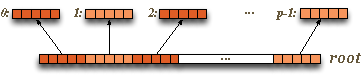
\includegraphics[scale=1.0]{figures/mpi-scatter.pdf}
    \end{figure}
%
  \item it is as if the data in \identifier{send\_buffer} were split in $p$ segments, and the
    \th{i} process receives the \th{i} segment
%
  \item the \identifier{send\_xxx} arguments are only meaningful for \identifier{root}; they
    are ignored for other processes
%
  \item the arguments \identifier{root} and \identifier{communicator} must be passed identical
    values by all processes
%
  \end{itemize}
% 
\end{frame}

% --------------------------------------
% gather
\begin{frame}[fragile]
%
  \frametitle{Gather}
%
  \begin{itemize}
%
  \item the converse is \function{MPI\_Gather} with \identifier{root} receiving data from all
    processes
    \begin{C}
int MPI_Gather(
        void* send_buffer, int send_count, MPI_Datatype send_datatype,
        void* recv_buffer, int recv_count, MPI_Datatype recv_datatype,
        int root, MPI_Comm communicator
        );
   \end{C}
   \begin{figure}
     \centering
     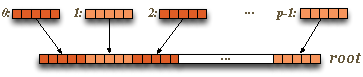
\includegraphics[scale=1.0]{figures/mpi-gather.pdf}
   \end{figure}
%
  \item it is as if $p$ messages, one from each processes, were concatenated in rank order and
    placed at \identifier{recv\_buffer}
%
  \item the \identifier{recv\_xxx} arguments are only meaningful for \identifier{root}; they
    are ignored for other processes
%
  \item the arguments \identifier{root} and \identifier{communicator} must be passed identical
    values by all processes
%
  \end{itemize}
%
\end{frame}

% --------------------------------------
% broadcasts
\begin{frame}[fragile]
%
  \frametitle{Broadcasting operations}
%
  \begin{itemize}
%
  \item \function{MPI\_Alltoall} sends data from all processes to all processes in a global
    scatter/gather
    \begin{C}
int MPI_Alltoall(
        void* send_buffer, int send_count, MPI_Datatype send_datatype,
        void* recv_buffer, int recv_count, MPI_Datatype recv_datatype,
        MPI_Comm communicator
        );
   \end{C}
%
 \item use \function{MPI\_Bcast} to send the contents of a buffer from \identifier{root} to all
   processes in a communicator
   \begin{C}
int MPI_Bcast(
        void* buffer, int count, MPI_Datatype datatype,
        int root, MPI_Comm communicator
        );
   \end{C}
%
  \end{itemize}
%
\end{frame}

% --------------------------------------
% collective operations summary
\begin{frame}[fragile]
%
  \frametitle{Data movement patterns for the collective operations}
%
  \begin{tabular}{cc}
    \parbox[c][1in]{2in}{
      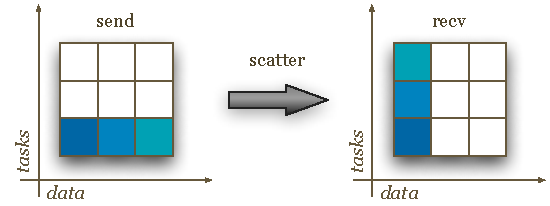
\includegraphics[scale=0.5]{figures/mpi-scatter-pattern.pdf}
    }
    &
    \parbox[c][1in]{2in}{
      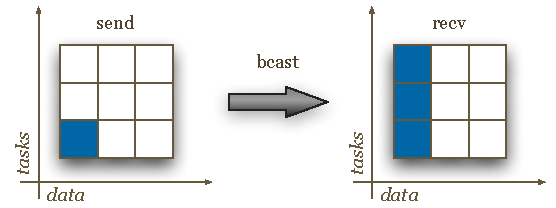
\includegraphics[scale=0.5]{figures/mpi-bcast-pattern.pdf}
    }
    \\ 
    \parbox[c][1in]{2in}{
      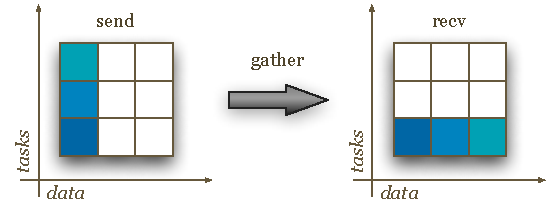
\includegraphics[scale=0.5]{figures/mpi-gather-pattern.pdf}
    }
    &
    \parbox[c][1in]{2in}{
      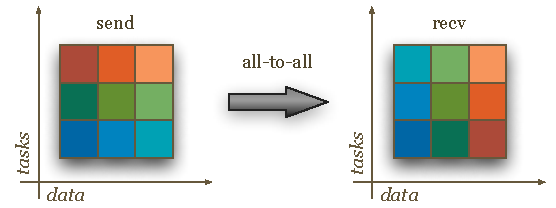
\includegraphics[scale=0.5]{figures/mpi-alltoall-pattern.pdf}
    }
  \end{tabular}
%
\end{frame}

% end of file
